\documentclass{article}
\usepackage{titling}
\usepackage{graphicx}
\usepackage{pgfgantt}
\usepackage{pdflscape}
\usepackage{hyperref}
\usepackage{animate}
\usepackage{movie15}
\usepackage[absolute,overlay]{textpos}
\usepackage{xspace}
\usepackage{subcaption}
\usepackage{listings}
\usepackage{amsmath}
\usepackage{caption}
\usepackage{enumitem}
\pretitle{
  \begin{center}
  \LARGE\bfseries
  
\includegraphics[width=0.2\textwidth]{image/logo (2).png} % Başlık önüne ekleyeceğiniz bir logo
  \vskip 1em
}
\title{Python ile Derin Öğrenme Kullanarak Otonom Bir Araba Oluşturmak}
\author{Ali Kağan Uyanık}
\date{Haziran 2024}



\begin{document}

\begin{titlingpage}
    \maketitle
    \begin{center}
        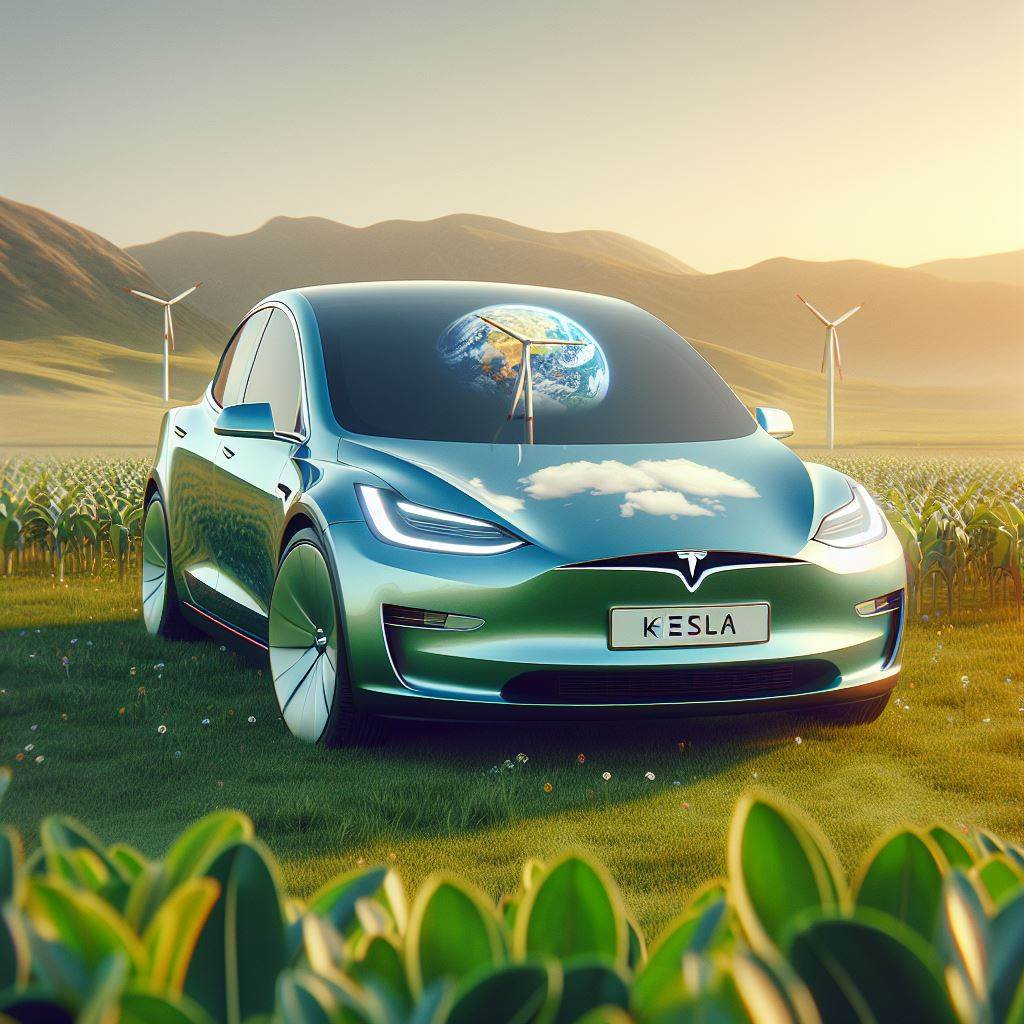
\includegraphics[width=0.6\textwidth]{image/otomobil.jpg} % Araba resminin dosya adını belirtin
    \end{center}
    \vfill
    
    \renewcommand{\abstractname}{Özet}
    \begin{abstract}
        \noindent Bu rapor,NVIDIA'nın Konvolüsyonel Sinir Ağı(CNN) mimarisi ve Udacity Simülatörü kullanılarak geliştirilen bir otonom araç modelinin uygulaması bulunmaktadır.Model,simüle edilmiş bir ortamda otonom olarak navigasyon yapabilmesi için eğitilmiştir.Bu çalışma,derin öğrenmenin otonom araçlar alanındaki yeteneklerini göstermektedir.
    \end{abstract}
    
    \vfill
\end{titlingpage}
\newpage

\section{Doğrudan Algılama (Direct Perception)}
Direct Perception yaklaşımı,otonom araçların çevresel bilgileri doğrudan algılayarak sürüş kararları almasını sağlar.Bu yaklaşımda,araçlar çevredeki nesneleri doğrudan algılar ve bu algılamalara dayanarak sürüş kararları alır.Kameralar,LIDAR,radar gibi sensörler aracılığıyla çevresel bilgiler toplanır ve yapay zeka algoritmalarıyla işlenir.Bu sayede araçlar,güvenli ve etkili bir şekilde sürüş yapabilir.

\begin{figure}[h]
  \centering
  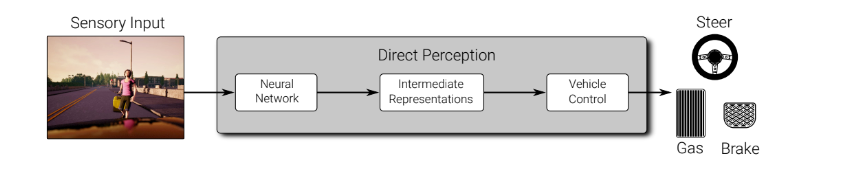
\includegraphics[width=1.1\textwidth]{image/Resim59.PNG} % Resim dosyasının adını ve uzantısını belirtin
\caption{Doğrudan Algılama \cite{Imitation}}
  \label{fig:cnnmimari}  
\end{figure}
\subsection{Davranışsal Klonlama(Behavioral Cloning)}
\subsubsection{Davranış Klonlamayı Anlamak}
Davranışsal klonlama,otonom araç sistemlerinde kullanılan bir yöntemdir.Bu yöntemde,bir insanın veya bir uzmanın aracın kontrolünü üstlendiği ve aracın belirli bir görevi yerine getirmesini sağladığı durumlar kaydedilir.Daha sonra,bu kaydedilen veriler kullanılarak bir yapay zeka modeli eğitilir.Bu model,insanın veya uzmanın yaptığı hareketleri ve kararları taklit etmeye çalışır.Sonuç olarak,otonom araçlar bu modeli kullanarak insan benzeri davranışları sergileyebilir ve belirli görevleri yerine getirebilir.

\begin{figure}[h]
  \centering
  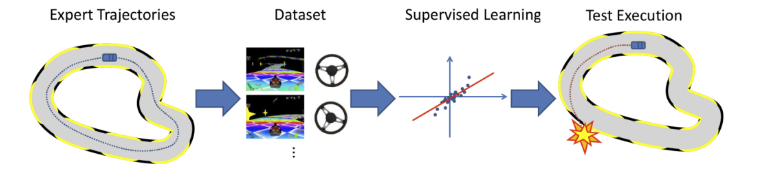
\includegraphics[width=1.1\textwidth]{image/Resim58.PNG} % Resim dosyasının adını ve uzantısını belirtin
\caption{Taklit Öğrenimi(Imitation Learning]\cite{Imitation}}
  \label{fig:cnnmimari}  
\end{figure}

\subsubsection{DAgger Yöntemi}
DAgger, otonom araç sistemlerinde kullanılan bir öğrenme yöntemidir. Bu yöntem, insan denetiminde aracın gerçek dünya deneyimlerinden sürekli olarak öğrenmesini sağlar. İşleyişi oldukça basittir: İnsan bir görevi yerine getirirken araç denetlenir, veri toplanır, makine öğrenimi algoritmaları kullanılarak öğrenme gerçekleştirilir, denetimsiz öğrenme süreci başlatılır, veri agregasyonu yapılır ve sürekli geri bildirim alınarak iyileştirmeler yapılır.


\begin{figure}[h]
  \centering
  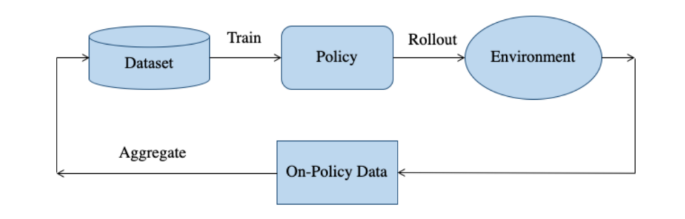
\includegraphics[width=1.1\textwidth]{image/Resim60.PNG} % Resim dosyasının adını ve uzantısını belirtin
\caption{DAgger'ın işleyişi\cite{prakash2020exploring}}
  \label{fig:cnnmimari}  
\end{figure}

\subsection{Deneysel Koşullar}
\subsubsection{Sürüş Simülatörü: Udacity}
Udacity'nin otonom araç simülatörü\cite{Udacity}, öğrencilere otonom araç yazılımını geliştirme fırsatı sunar.Gerçek dünya senaryolarını taklit eden bir ortam sağlar,böylece öğrenciler pratik yapabilir,hata ayıklayabilir ve becerilerini geliştirebilirler.Bu simülatör,öğrencilere gerçek dünya deneyimi kazandırırken maliyetleri ve riskleri azaltır.\\[2pt]
Simülatör iki pist içerir.Bunlardan biri basit olarak kabul edilebilirken diğeri karmaşıktır.Buradaki "basit" kelimesi,daha az kavisli pistlere sahip olduğu ve sürüşün daha kolay olduğu anlamına gelir.Simülatörde aracı sürmenin iki modu bulunmaktadır:(1) Eğitim modu ve (2) Otonom mod.Eğitim modu,sürüşünüzü kaydetme ve eğitim veri setini yakalama seçeneği sunar.\\[1pt]

\begin{figure}[h]
    \centering
    \begin{subfigure}{0.5\textwidth}
        \centering
        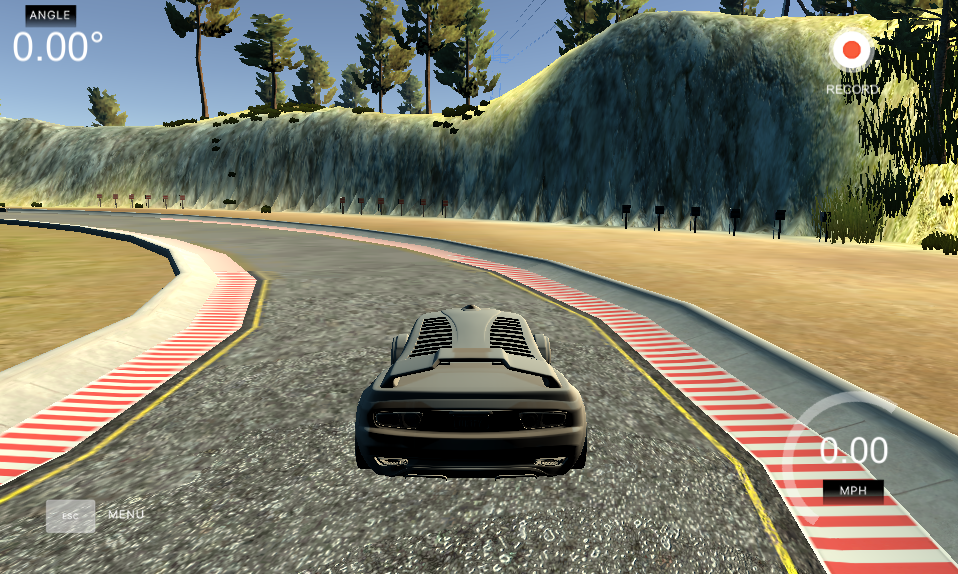
\includegraphics[width=1.1\linewidth]{image/Resim61.PNG}
        \caption{Basit Pist}
        \label{fig:resim1}
    \end{subfigure}%
    \begin{subfigure}{0.5\textwidth}
        \centering
        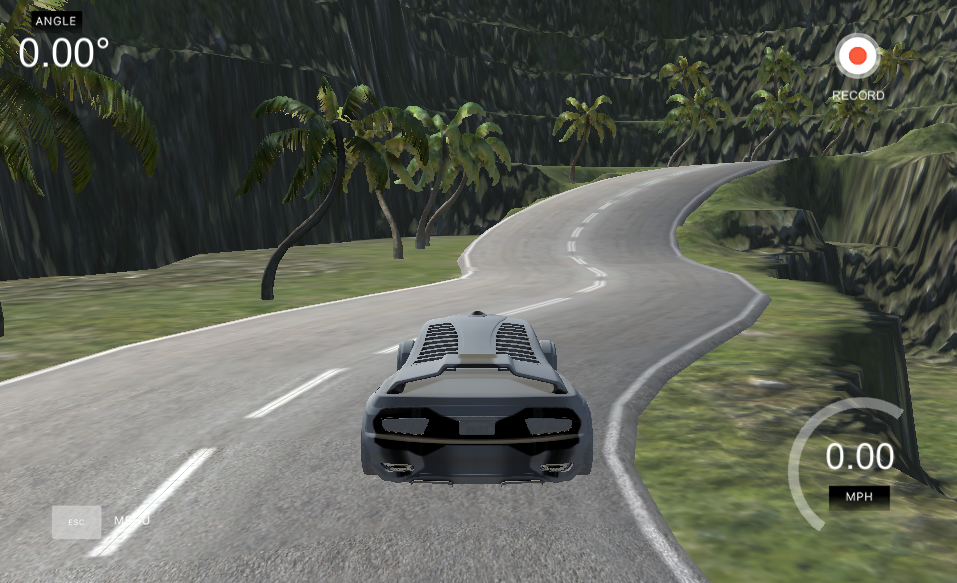
\includegraphics[width=1.1\linewidth]{image/Resim62.PNG}
        \caption{Karmaşık Pist}
        \label{fig:resim2}
    \end{subfigure}
    \label{fig:iki_resim}
\end{figure}
\newpage
\subsubsection{Veri Toplama}
Süreci başlatmak için bir otonom araç simülatörü kullanılır. Bu simülatör,Udacity gibi bir kaynaktan sağlanan, belirlenen pistlerde sanal bir araçla sürüş yaparak eğitim verisi oluşturmayı sağlar.Simülatörün kendi görüntü veri setinizi oluşturma özelliği, sorun üzerinde çalışmayı kolaylaştırır. Bu özelliğin faydalı olmasının bazı nedenleri şunlardır:
\begin{itemize}
    \item Simülatör,arabanın üstünde üç kamera olduğunu simüle edecek şekilde sürüş özelliklerini oluşturmuştur.Bu üç kamera, arabayın önünde merkezde,sağda ve solda bulunur ve eğitim modunda kayıt yaptığımızda sürekli olarak görüntüleri yakalar.
    \item Görüntü akışı yakalanır ve kayıt düğmesine bastıktan sonra verilerin kaydedileceği disk konumu ayarlanabilir.Görüntü setleri,hangi kameradan görüntünün yakalandığını belirten merkez,sol veya sağ ön ekleri ile sofistike bir şekilde etiketlenmiştir.
    \item Görüntü veri setinin yanı sıra,ayrıca bir \texttt{datalog.csv} dosyası oluşturur.Bu dosya, o anki görüntü yollarını ve ilgili direksiyon açısını,gazı,frenleri ve arabanın hızını içerir.
\end{itemize}
\begin{figure}[h]
  \centering
  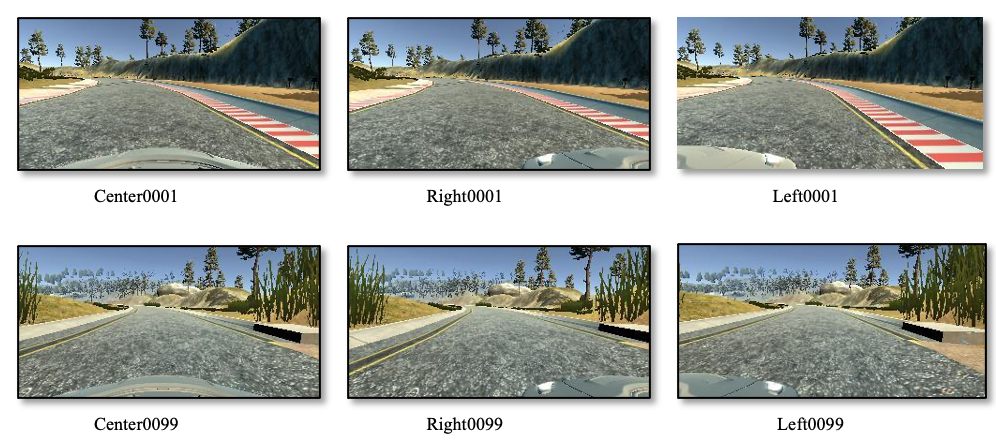
\includegraphics[width=1.1\textwidth]{image/5..png} % Resim dosyasının adını ve uzantısını belirtin
\caption{Veri Toplama}
  \label{fig:cnnmimari}  
\end{figure}
\subsubsection{Veri Dağılımını Optimize Etme}
Kendi kendine sürüş arabası projesinde, eğitim verilerimin düz gitmeye meyilli olduğunu fark ettim. Bu durum, modelimin sürekli olarak düz gitmeye yönelik bir eğilim geliştirmesine neden olabilir. Bu sorunu çözmek için, arabamın meydan okuma pistinde güvenilir bir şekilde gezinebilmesi için bazı ön işleme tekniklerini uygulayacağım.

\noindent Veri dağılımımı düzleştirmeli ve 200'ü aşan frekanslara sahip kutulardan gereksiz örnekleri kaldırmam gerekiyor.Böylece, veri dağılımımı optimize ederek modelimi daha etkili bir şekilde eğitmek için hazırlıklı oluyorum.

\begin{figure}[h]
  \centering
  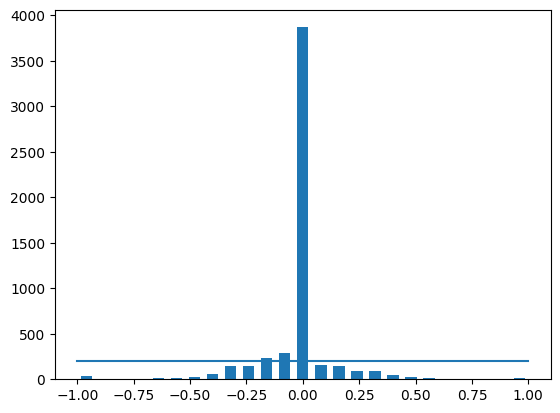
\includegraphics[width=0.8\textwidth]{image/grafik.png} % Resim dosyasının adını ve uzantısını belirtin
\caption{Veri dağılımını optimize etme}
  \label{fig:cnnmimari}  
\end{figure}





\subsubsection{Eğitim ve Doğrulama Ayrımı}
Bu kısımda,otonom sürüş için bir yapay zeka modeli eğitmeden önce veri hazırlığı yapılmıştır.İlk olarak, veri yüklenir ve görüntü dosyaları ile bunlara karşılık gelen direksiyon açıları depolanır.Daha sonra, veri rastgele eğitim ve doğrulama veri kümelerine bölünür.Her iki veri kümesi için de yönlendirme açılarının dağılımı kontrol edilir ve bunlar histogramlarla görselleştirilir.

\begin{figure}[h]
  \centering
  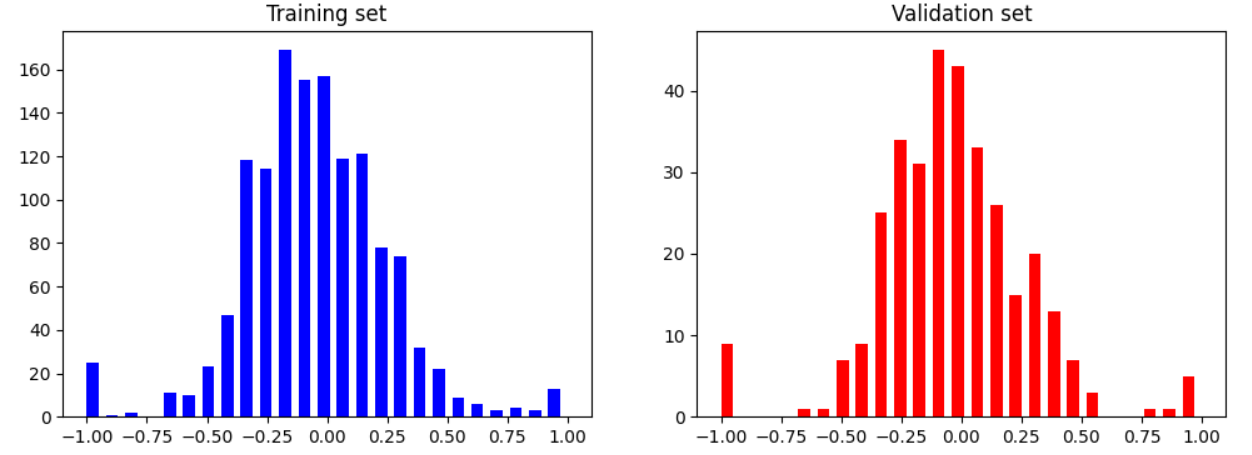
\includegraphics[width=1\textwidth]{image/Resim64.PNG} % Resim dosyasının adını ve uzantısını belirtin
\caption{Veri Toplamadaki Zorluklar}
  \label{fig:cnnmimari}  
\end{figure}
\newpage

\subsubsection{Bazı Artırma Tekniklerinin Uygulanması(Data Augmentation)}
Otonom araç yapay zeka modelimin dayanıklılığını ve genelleme yeteneğini artırmak için çeşitli veri artırma teknikleri kullandım.Veri artırma,derin öğrenme modellerinin eğitimi sırasında özellikle görsel verilerle çalışırken kritik bir süreçtir,çünkü daha fazla veri toplamaya gerek kalmadan eğitim veri setinin boyutunu yapay olarak genişletmeye yardımcı olur.Bu yaklaşım,mevcut veri örneklerine bir dizi dönüşüm uygulayarak farklı sürüş koşullarını ve senaryolarını simüle etmeyi içerir.İşte kullandığım bazı temel artırma teknikleri:\\[5pt]
\textbf{Ölçekleme ve Kırpma:} Ölçekleme ve kırpma,aracın görüş açısındaki nesnelere daha yakın veya uzak olmasını simüle etmek için kullanılır.Bu,modelin farklı mesafelerdeki nesnelerin nasıl görünebileceğini öğrenmesi açısından özellikle faydalıdır ve algılanan mesafelere dayalı olarak uygun direksiyon açılarını tahmin etme yeteneğini artırır.Kırpma ayrıca modelin dikkatini görüntünün ilgili bölümlerine,örneğin yol veya engellere,odaklamasına yardımcı olur. \\
\begin{figure}[h]
  \centering
  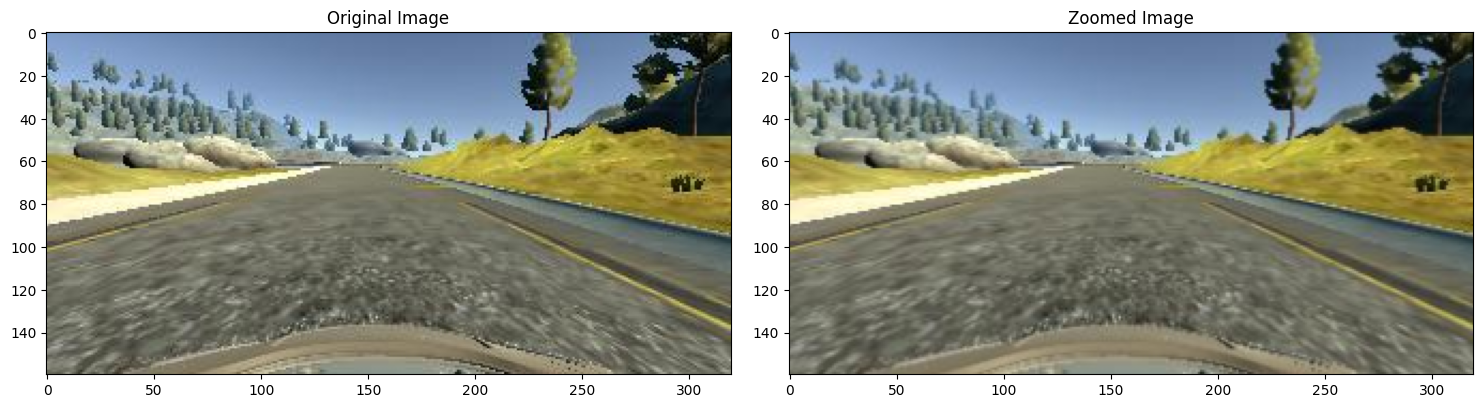
\includegraphics[width=1\textwidth]{image/1..png} % Resim dosyasının adını ve uzantısını belirtin
\caption{Orijinal Görüntü/Yakınlaştırılmış Görüntü}
  \label{fig:cnnmimari}  
\end{figure}
\newline
\textbf{Parlaklık ve Kontrast Ayarı:} Görüntülerin parlaklık ve kontrast ayarları;alacakaranlık, şafak veya bulutlu hava gibi farklı aydınlatma koşullarını simüle eder.Bu,modelin günün saati veya hava durumu gibi sürüş görünürlüğünü ve güvenliğini etkileyebilecek yaygın değişkenlerden bağımsız olarak etkili kalmasını sağlar. 
\begin{figure}[h]
  \centering
  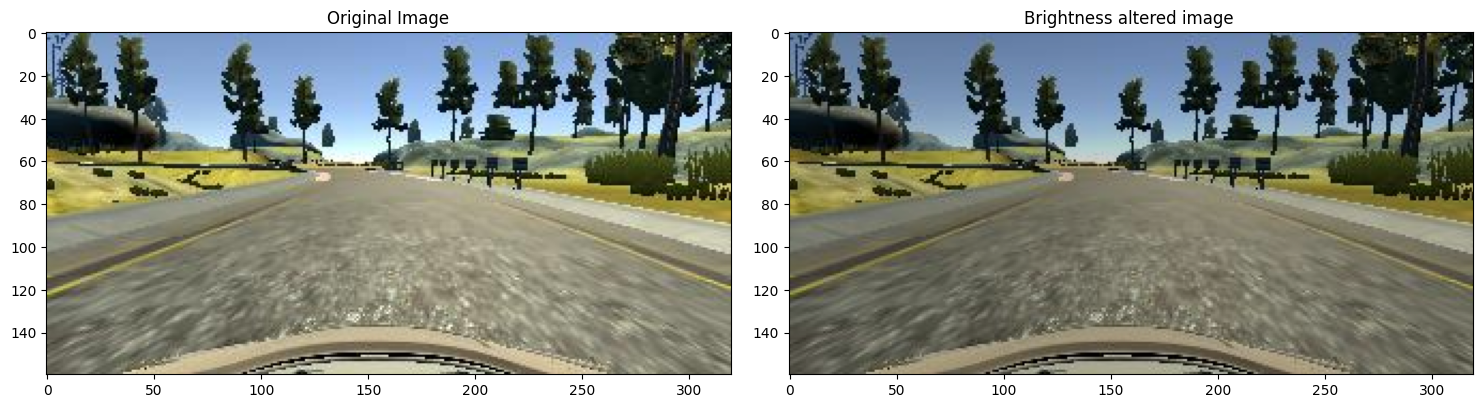
\includegraphics[width=1\textwidth]{image/2..png} % Resim dosyasının adını ve uzantısını belirtin
\caption{Orijinal Görüntü/Parlaklığı Değiştirilmiş Görüntü}
  \label{fig:cnnmimari}  
\end{figure}
\newpage

\textbf {\noindent Görüntüleri Yatay Çevirme:} Bu teknik,veri setinin boyutunu etkili bir şekilde iki katına çıkarır ve modelin bir yönde daha sık dönüş yapma eğilimi geliştirmemesini sağlamak için özellikle faydalıdır.Görüntüleri yatay olarak çevirerek,karşıt direksiyon yönünü simüle edebilir ve modelin sol ve sağ dönüşleri simetrik bir şekilde ele almayı öğrenmesini sağlayabiliriz. \\
\begin{figure}[h]
  \centering
  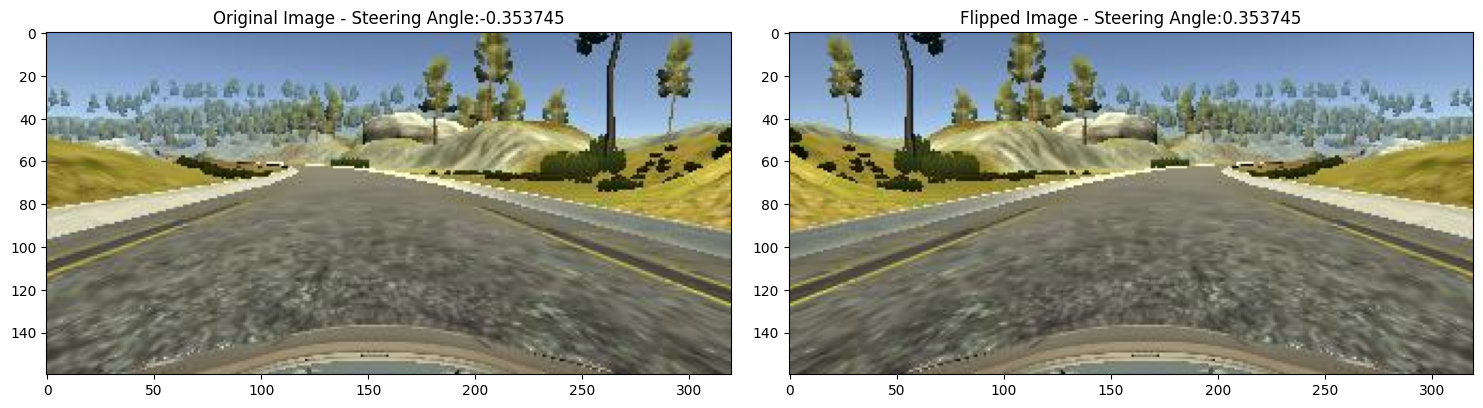
\includegraphics[width=1\textwidth]{image/3..png} % Resim dosyasının adını ve uzantısını belirtin
\caption{Orijinal Görüntü- Direksiyon Açısı/Ters Döndürülmüş Görüntü - Direksiyon Açısı}
  \label{fig:cnnmimari}  
\end{figure}

\textbf {Kaydırma:} Kaydırma,görüntüyü yatay veya dikey olarak kaydırmayı içerir ve aracın şerit içinde hareket etmesini veya yolun hizalanmasına göre ayarlamalar yapmasını simüle etmek için gereklidir.Bu,özellikle aracın şerit içinde hafif pozisyonel ayarlamalar yapması gerektiği,engellerden kaçınmak veya yola daha iyi hizalanmak için gerekli olan senaryoları öğretmek açısından faydalıdır.Kaydırma,giriş verilerinin değişkenliğini artırır ve modelin gerçek dünyadaki sürüşte yaygın bir gereklilik olan küçük pozisyonel ayarlamaları ele alacak şekilde iyi eğitilmesini sağlar. \\

\begin{figure}[h]
  \centering
  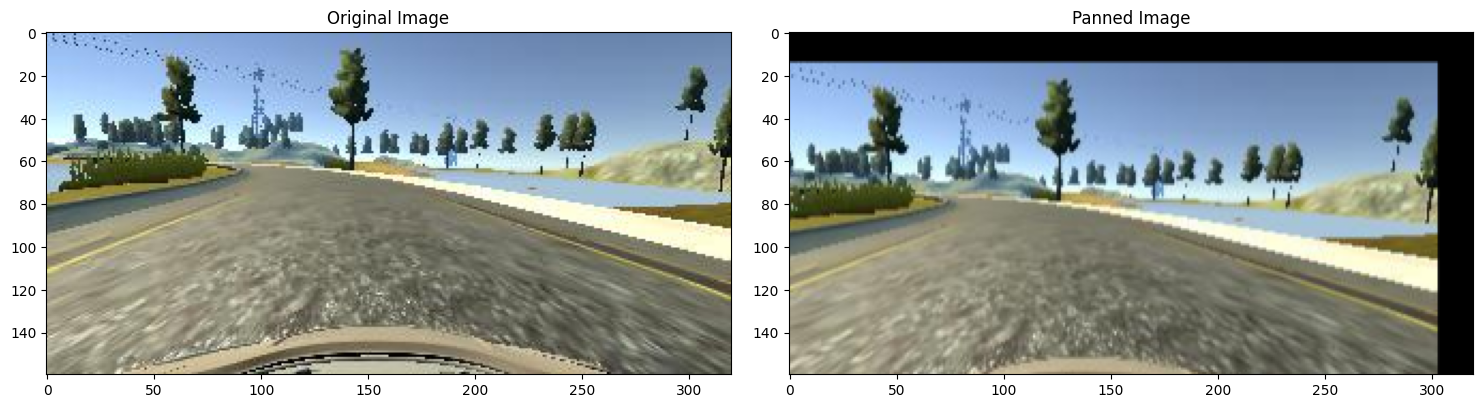
\includegraphics[width=1\textwidth]{image/4..png} % Resim dosyasının adını ve uzantısını belirtin
\caption{Orijinal Görüntü/Kaydırılan Görüntü}
  \label{fig:cnnmimari}  
\end{figure}

Bu artırma tekniklerini uygulayarak,daha sağlam ve doğru bir modelin eğitilmesine yardımcı olacak çeşitli senaryoları yapay olarak oluşturabiliriz. Bu yaklaşım,modelin daha geniş bir potansiyel gerçek dünya koşulları spektrumunda eğitilmesi nedeniyle aşırı öğrenme riskini önemli ölçüde azaltır ve gerçek sürüş ortamında dağıtıldığında daha uyumlu ve güvenilir hale getirir.

\subsubsection{Görüntülerin Ön İşleme Alınması}
\textbf{Görüntü Okuma:} İşlenecek olan görüntü dosyası okunur ve bir matrise dönüştürülür. Bu adım, işleme öncesinde temel veri yapısını oluşturur. \\
\textbf{ROI Seçimi:} ROI (Region of Interest - İlgilenilen Bölge), görüntü üzerinde işleme yapılacak bölgenin belirlenmesidir. Genellikle, gereksiz bilgileri filtrelemek veya yalnızca belirli bir bölgeye odaklanmak için yapılır. \\
\textbf{Renk Uzayı Dönüşümü:} Görüntü, farklı renk uzaylarına dönüştürülerek işlem kolaylığı sağlanır veya belirli özellikler vurgulanır. Örneğin, RGB uzayından YUV uzayına dönüşüm, parlaklık ve renk bilgisini daha ayrıntılı olarak ayırabilir. \\
\textbf{Gauss Filtresi Uygulama:} Gauss filtresi, gürültüyü azaltmak veya kenarları yumuşatmak için kullanılır. Görüntü üzerindeki istenmeyen piksel dalgalanmalarını azaltır. \\
\textbf{Boyutlandırma ve Normalizasyon:} Görüntü, belirli boyutlara yeniden boyutlandırılır ve ardından piksel değerleri [0, 1] aralığına normalleştirilir. Bu adımlar, işleme için girdi verisinin tutarlılığını sağlar.
\begin{figure}[h]
  \centering
  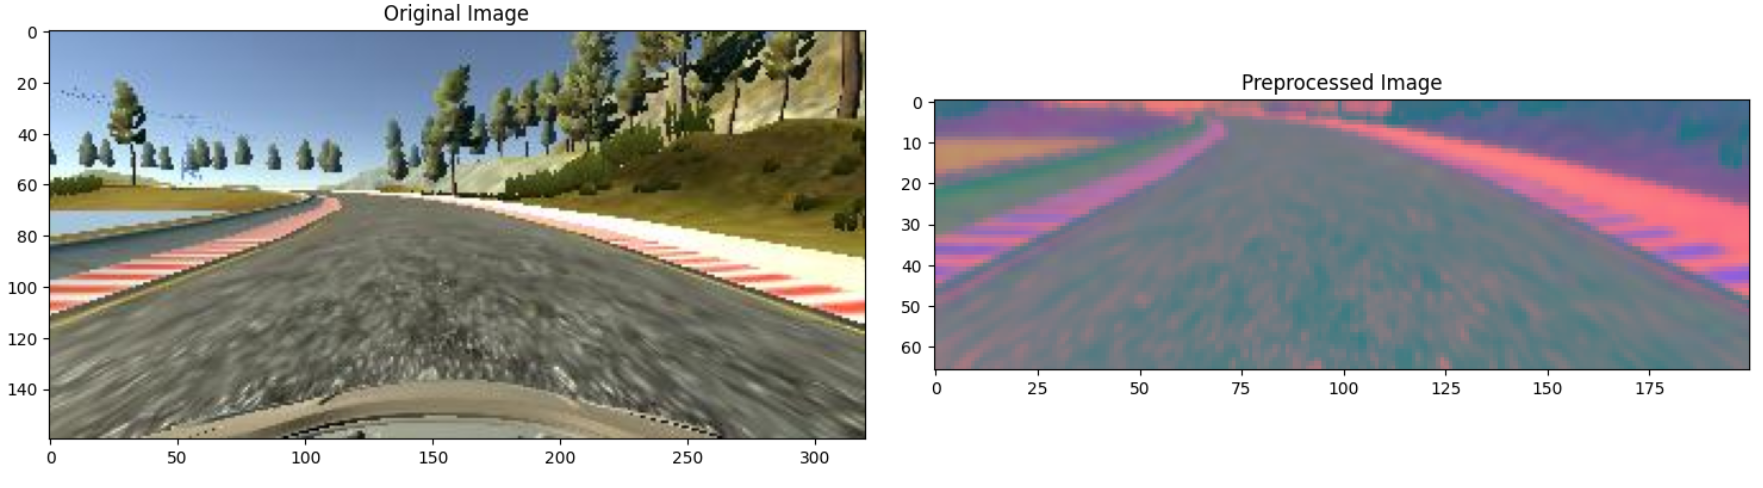
\includegraphics[width=1\textwidth]{image/Resim65.PNG} % Resim dosyasının adını ve uzantısını belirtin
\caption{Orijinal Görüntü ve Ön İşleme Sonu Görüntü}
  \label{fig:cnnmimari}  
\end{figure}

\subsubsection{Nvidia Model (PilotNet)}
Sürücüsüz araç hareket halindeyken aracın üç kamerasından toplanan görüntüler rastgele kaydırılır ve döndürülür ardından sinir ağı beslenir. Bu girdilere dayanarak, sinir ağı tek bir değer, direksiyon açısını üretir.Temel olarak, giriş görüntülerine dayanarak, sinir ağı aracın hangi açıdan yönlendirilmesi gerektiğine karar verir.Bu çıktı değeri, sinir ağının kararındaki hatayı hesaplamak için insan sürüşünden toplanan direksiyon verileriyle karşılaştırılır.Model, bu hatayı azaltmak için ağırlıkları geriye yayılım algoritmasını kullanarak günceller.
\begin{figure}[h]
  \centering
  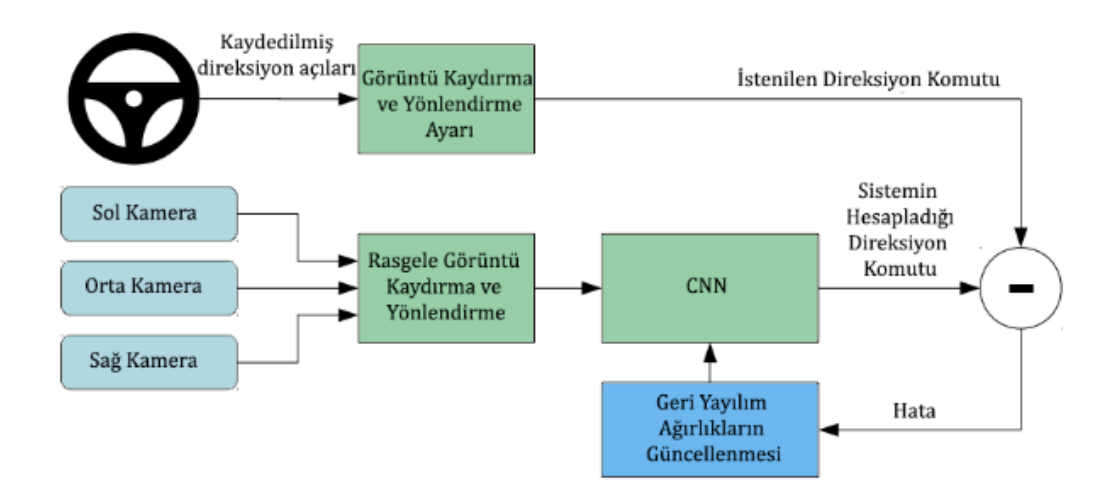
\includegraphics[width=1\textwidth]{image/Resim66.PNG} % Resim dosyasının adını ve uzantısını belirtin
\caption{Sürücüsüz Araç için CNN Eğitimi\cite{bojarski2016end}.}
  \label{fig:cnnmimari}  
\end{figure}
\newpage
\begin{document}

PilotNet modeli, dokuz katmandan oluşur:

\begin{itemize}
    \item Beş Evrişimli Katman (Convolutional Layers): Bu katmanlar, Evrişimli Sinir Ağı (CNN) adı verilen bir yapı oluşturur. Temel olarak, bu katmanlar görüntüleri işleyerek özelliklerin eğitimini sağlar. Görüntülerin farklı özelliklerini çıkarmak için özel filtreler kullanılır ve bu filtrelerin öğrenilmesi, modelin görüntü verilerinden anlam çıkarmasını sağlar.
    
    \item Üç Yoğun Katman (Dense Layers): Bu katmanlar, önceki evrişimli katmanlardan gelen özellikleri daha yüksek seviyede birleştirir ve derin öğrenme modelinin daha karmaşık ilişkileri öğrenmesine olanak tanır. Yoğun katmanlar, önceki katmanların çıkardığı özellikleri kullanarak sınıflandırma veya regresyon gibi belirli görevleri yerine getirmek için kullanılır.
    
    \item Çıkış Katmanı (Output Layer): Çıkış katmanı, modelin son tahminini veya çıktısını oluşturur. Otomatik sürüş durumunda, bu genellikle aracın yönlendirilmesiyle ilgili bilgileri içerir. Örneğin, aracın direksiyon açısını belirleyen bir regresyon çıktısı veya aracın farklı manevralarını temsil eden bir sınıflandırma çıktısı olabilir. Çıkış katmanı, modelin öğrenme sürecinin sonunda en önemli kararları verir ve eğitim sırasında modelin performansını değerlendirmede kullanılır.\\[1pt]
\end{itemize}
\newpage
\begin{figure}[h]
  \centering
  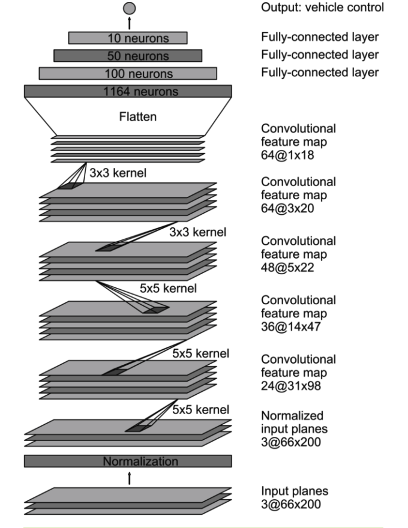
\includegraphics[width=0.8\textwidth]{image/Resim67.PNG} % Resim dosyasının adını ve uzantısını belirtin
\caption{Ağ Düzeni\cite{bojarski2016end}.}
  \label{fig:cnnmimari}  
\end{figure}

\subsubsection{Otonom Sürüş İçin Deneysel Yapılandırmalar}
Simülasyon için güçlü ve etkili bir sinir ağı modeli geliştirmek için çeşitli deneysel yapılandırmalar keşfedilmiş ve titizlikle test edilmiştir.Bu kısım, bu deneylerden türetilen optimal yapılandırmayı, model mimarisi, veri kümesi kullanımı, eğitim parametreleri ve performansı artırmak için yapılan ayarları içerir.
\newpage


\subsection*{Veri Kümesi Kullanımı}
\begin{itemize}
    \item Modeller yalnızca Track 1'den gelen verilerle eğitilmiştir.
    \item Veri bölünmesi: Eğitim için \%80, test için \%20.
\end{itemize}

\subsection*{Eğitim Parametreleri}
\begin{itemize}
    \item Epochlar: 10 (overfitting'i önlemek için)
    \item Batch Boyutu: 100 (veri yayılması için verimli)
    \item Öğrenme Oranı: 0.0001 (ağırlık ayarlamalarını optimize etmek için)
\end{itemize}

\subsection*{Ağ Mimarisi}
Model mimarisi, end-to-end sürüş testlerindeki etkinliğiyle tanınan NVIDIA modelinden ilham alınarak oluşturulmuştur. Modeli projenin gereksinimlerine uygun hale getirmek ve performansını artırmak için temel ayarlamalar yapılmıştır.

\subsection*{Yapılan Ayarlamalar}
\begin{enumerate}
    \item \textbf{Giriş Normalizasyonu:} Giriş görüntülerini normalize etmek için Lambda katmanının kullanılması, doygunluğu önler ve daha iyi gradyan işleyişini sağlar.
    \item \textbf{Dropout Katmanı:} Overfitting'i önlemek için konvolüsyon katmanları sonrasına ek bir dropout katmanı eklenmiştir.
    \item \textbf{Aktivasyon Fonksiyonu:} Her katmanda, çıktı katmanı hariç, doğrusal olmayanlık eklemek ve tahmin doğruluğunu artırmak için Exponential Linear Unit (ELU) aktivasyonu kullanılmıştır.
\end{enumerate}

\subsection*{Optimal Model Yapılandırması}
\begin{enumerate}
    \item Giriş Normalizasyonu
    \item Konvolüsyon: 5x5, Filtre: 24, Adımlar: 2x2, Aktivasyon: ELU
    \item Konvolüsyon: 5x5, Filtre: 36, Adımlar: 2x2, Aktivasyon: ELU
    \item Konvolüsyon: 5x5, Filtre: 48, Adımlar: 2x2, Aktivasyon: ELU
    \item Konvolüsyon: 3x3, Filtre: 64, Adımlar: 1x1, Aktivasyon: ELU
    \item Konvolüsyon: 3x3, Filtre: 64, Adımlar: 1x1, Aktivasyon: ELU
    \item Dropout (0.5)
    \item Tam Bağlantı: Nöronlar: 100, Aktivasyon: ELU
    \item Tam Bağlantı: Nöronlar: 50, Aktivasyon: ELU
    \item Tam Bağlantı: Nöronlar: 10, Aktivasyon: ELU
    \item Tam Bağlantı: Nöronlar: 1 (Çıkış)
\end{enumerate}

\begin{table}[htbp]
  \centering
  \resizebox{\textwidth}{!}{%
  \begin{tabular}{|c|c|c|}
  \hline
  \textbf{Layer (type)} & \textbf{Output Shape} & \textbf{Param} \\
  \hline
  Conv2D & (None, 31, 98, 24) & 1824 \\
  Conv2D & (None, 14, 47, 36) & 21636 \\
  Conv2D & (None, 5, 22, 48) & 43248 \\
  Conv2D & (None, 3, 20, 64) & 27712 \\
  Conv2D & (None, 1, 18, 64) & 36928 \\
  Dropout & (None, 1, 18, 64) & 0 \\
  Flatten & (None, 1152) & 0 \\
  Dense & (None, 100) & 115300 \\
  Dropout & (None, 100) & 0 \\
  Dense & (None, 50) & 5050 \\
  Dropout & (None, 50) & 0 \\
  Dense & (None, 10) & 510 \\
  Dropout & (None, 10) & 0 \\
  Dense & (None, 1) & 11 \\
  \hline
  \end{tabular}%
  }
  \caption{Model Mimarisi}
  \label{tab:model_architecture}
\end{table}

\section*{Sonuç}
Titiz deneyler ve parametre ayarlamalarının sonucunda, simülasyon için optimal bir sinir ağı yapılandırması tanımlanmıştır.Derin konvolüsyon katmanlarından, dropout düzenlemesinden faydalanarak,model gelişmiş performans ve sağlamlık sergiler,böylelikle simüle ortamlarda etkili otonom sürüş için yol açılır.\newpage

\begin{figure}[htbp]
  \centering
  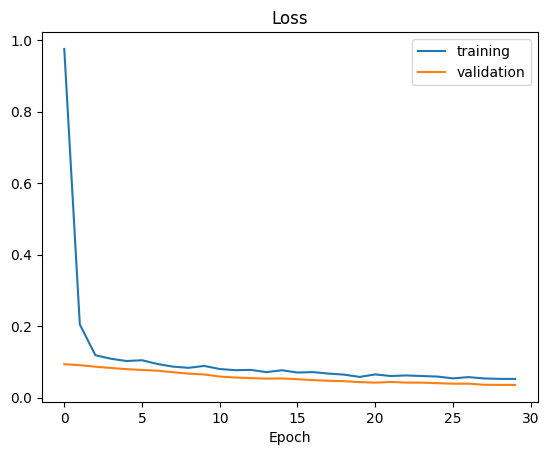
\includegraphics[width=1\textwidth]{image/Resim68.png} % Resmin dosya adı example-image, bu kısmı kendi resminizin adıyla değiştirin
  \caption{Kayıp (loss) değerlerinin eğrisi}
  \label{fig:resim_etiketi}
\end{figure}

Taban alınan simülasyon temelli değerlendirmeler,modelin pratik uygulanabilirliği ve güvenliğini gerçek dünya koşullarında test etme imkanı sağlamıştır.Udacity simülatöründeki olumlu sonuçlar,modelin ileri geliştirme aşamaları ve potansiyel gerçek dünya kullanımları için uygun olduğunu göstermektedir.Bu bulgular,modelin sanal ortamda güvenilir performans sergilediği ve gelecekte gerçek dünya uygulamalarında başarılı olabileceği umudunu güçlendirmektedir.

\section*{Gelecekteki Çalışmalar}
\begin{itemize}[leftmargin=*] % adjust leftmargin as needed
    \item Modelin gerçek dünya koşullarında doğruluğunu ve güvenilirliğini doğrulamak için saha testleri yapılmalıdır.
    \item Modelin daha geniş bir veri setinde ve farklı çevresel koşullarda performansını değerlendirmek için testler genişletilmelidir.
    \item Daha karmaşık sürüş senaryolarını içeren simülasyonlarla modelin güvenlik ve adaptasyon yeteneklerini daha da güçlendirmek gereklidir.
    \item Eğitim sürecinde modelin hızını ve verimliliğini artırmak için optimize edilmiş algoritmalar ve donanımlar kullanılmalıdır.
\end{itemize}
\section*{Projeden Görüntüler}
\begin{figure}[htbp]
  \centering
  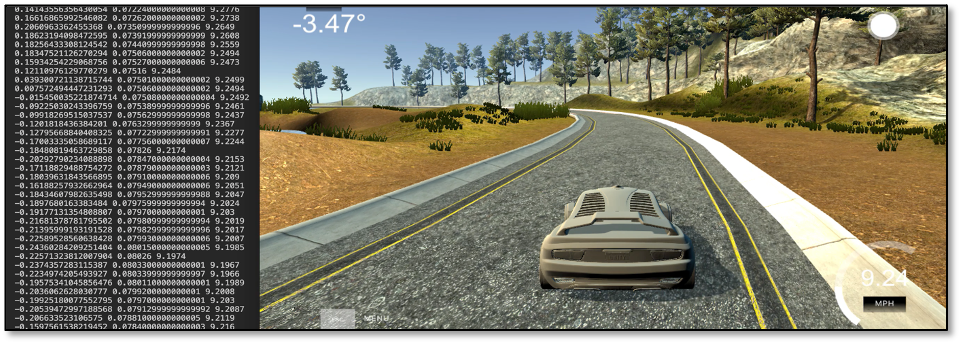
\includegraphics[width=1.1\textwidth]{image/6..png} % Resmin dosya adı example-image, bu kısmı kendi resminizin adıyla değiştirin
  \caption{Otonom Modda Sürüş}
  \label{fig:resim_etiketi}
\end{figure}

\bibliographystyle{ieeetr}
\bibliography{referans}
\end{document}
